% Homework template for Learning from Data
% by Xiangxiang Xu <xiangxiangxu.thu@gmail.com>
% LAST UPDATE: October 8, 2018
\documentclass[a4paper]{article}
\usepackage[T1]{fontenc}
\usepackage{amsmath, amssymb, amsthm}
% amsmath: equation*, amssymb: mathbb, amsthm: proof
\usepackage{moreenum}
\usepackage{mathtools}
\usepackage{url}
\usepackage{enumitem}
\usepackage{bm}
\usepackage{graphicx}
\usepackage{subcaption}
\usepackage{booktabs} % toprule
\usepackage[mathcal]{eucal}
\usepackage{dsfont}
\usepackage[numbered,framed]{matlab-prettifier}
%% Definitions for Learning from Data
%% UPDATE: October 8, 2018 by Xiangxiang 
\newcommand{\theterm}{Fall 2019}

\newcommand{\thecoursename}{
Tsinghua-Berkeley Shenzhen Institute\\
%\vspace*{0.1in}
\textsc{Learning from Data}
}

\newcommand{\courseheader}{
\vspace*{-1in}
\begin{center}
\thecoursename \\
\theterm
\vspace*{0.1in}
\hrule
\end{center}
}
\newcommand{\uc}{\underline{c}}    % c, vec
\newcommand{\uv}{\underline{v}}    % x, vec
\newcommand{\uw}{\underline{w}}    % w, vec
\newcommand{\ux}{\underline{x}}    % x, vec
\newcommand{\uy}{\underline{y}}    % y, vec
\newcommand{\uz}{\underline{z}}    % z, vec
\newcommand{\um}{\underline{m}}    % m, vec
\newcommand{\ut}{\underline{t}}    % t, vec
\newcommand{\bc}{\bm{c}}    % c, vec
\newcommand{\bv}{\bm{v}}    % x, vec
\newcommand{\bw}{\bm{w}}    % w, vec
\newcommand{\bx}{\bm{x}}    % x, vec
\newcommand{\by}{\bm{y}}    % y, vec
\newcommand{\bz}{\bm{z}}    % z, vec
% \newcommand{\bm}{\bm{m}}    % m, vec
\newcommand{\bt}{\bm{t}}    % t, vec

\newcommand{\balpha}{\bm{\alpha}}    % alpha, vec
\newcommand{\bxi}{\bm{\xi}}    % xi, vec


\newcommand{\rvx}{\mathsf{x}}    % x, r.v.
\newcommand{\rvy}{\mathsf{y}}    % y, r.v.
\newcommand{\rvz}{\mathsf{z}}    % z, r.v.
\newcommand{\rvw}{\mathsf{w}}    % w, r.v.
\newcommand{\rvv}{\mathsf{v}}    % v, r.v.
\newcommand{\rvm}{\mathsf{m}}    % m, r.v.
\newcommand{\rvt}{\mathsf{t}}    % t, r.v.
\newcommand{\rvH}{\mathsf{H}}    % H, r.v.
\newcommand{\urvx}{\underline{\mathsf{x}}}    % x, r.v. vec
\newcommand{\urvy}{\underline{\mathsf{y}}}    % y, r.v. vec
\newcommand{\urvz}{\underline{\mathsf{z}}}    % z, r.v. vec
\newcommand{\urvw}{\underline{\mathsf{w}}}    % w, r.v. vec
\newcommand{\urvt}{\underline{\mathsf{t}}}    % t, r.v. vec
\newcommand{\defeq}{\triangleq} %\coloneqq
\newcommand{\reals}{\mathbb{R}}
\newcommand{\T}{\mathrm{T}}    % transpose
\newcommand{\BLS}{\mathrm{BLS}}    % BLS
\newcommand{\LLS}{\mathrm{LLS}}    % LLS
\newcommand{\MVU}{\mathrm{MVU}}    % MVU

\DeclareMathOperator*{\maximize}{maximize}    % maximize
\DeclareMathOperator*{\minimize}{minimize}    % minimize
\newcommand{\st}{\mathrm{subject~to}}    % minimize


% \newcommand{\E}[1]{\mathbb{E}\left[{#1}\right]}
% \newcommand{\Prob}[1]{\mathbb{P}\left({#1}\right)}
\DeclareMathOperator*{\argmax}{arg\,max}
\DeclareMathOperator*{\argmin}{arg\,min}
\DeclareMathOperator*{\argsup}{arg\,sup}
\DeclareMathOperator*{\arginf}{arg\,inf}
\DeclareMathOperator{\Var}{Var}
\DeclareMathOperator{\Cov}{Cov}
\DeclareMathOperator{\MSE}{MSE}
\DeclareMathOperator{\1}{\mathds{1}}
\DeclareMathOperator{\E}{\mathbb{E}}
\DeclareMathOperator{\Prob}{\mathbb{P}}

\newcommand\independent{\protect\mathpalette{\protect\independenT}{\perp}}
\def\independenT#1#2{\mathrel{\rlap{$#1#2$}\mkern2mu{#1#2}}}


\lstset{
  style              = Matlab-editor,
  captionpos         =b,
  basicstyle         = \mlttfamily,
  escapechar         = ",
  mlshowsectionrules = true,
}
\begin{document}
\courseheader



\newcounter{hwcnt}
\setcounter{hwcnt}{1} % set to the times of Homework

\begin{center}
  \underline{\bf Homework \thehwcnt} \\
\end{center}
\begin{flushleft}
  TIAN Chenyu\hfill
  \today
\end{flushleft}
\hrule

\vspace{2em}
\setlist[enumerate,1]{label=\thehwcnt.\arabic*.}
\setlist[enumerate,2]{label=(\alph*)}
\setlist[enumerate,3]{label=\roman*.}
\setlist[enumerate,4]{label=\greek*)}

\flushleft
\rule{\textwidth}{1pt}
\begin{itemize}
\item {\bf Acknowledgments: \/} 
  This template takes some materials from course CSE 547/Stat 548 of Washington University: \small{\url{https://courses.cs.washington.edu/courses/cse547/17sp/index.html}}.
\item {\bf Collaborators: \/}
  I finish this template by myself.
  % \begin{itemize}
  % \item 1.2 (b) was solved with the help from \underline{\hspace{3em}}.
  % \item Discussion with \underline{\hspace{3em}} helped me finishing 1.3.
  % \end{itemize}
\end{itemize}
\rule{\textwidth}{1pt}

\vspace{2em}

% You may use \texttt{enumerate} to generate answers for each question:

\begin{enumerate}
  \setlength{\itemsep}{3\parskip}
\item Suppose the data are linearly separable. The optimization problem of SVM is  \begin{equation}
    \tag{P}
    \begin{aligned}
      &\minimize_{\bw, b}& &\frac12 \|\bw\|_2^2\\
      &\st& &y_i(\bw^{\T}\bx_i + b) \geq 1, \quad i = 1, \dots, l,
    \end{aligned}
    \label{eq:svm:p}
  \end{equation}
  and let $(\bw^{\star}, b^{\star})$ denote its optimal solution.
  \begin{enumerate}
  \item Show that
    \begin{equation*}
      b^{\star} = -\frac12 \left(\max_{i\colon y_i = -1}\bw^{\star\T}\bx_i + \min_{i\colon y_i = 1}\bw^{\star\T}\bx_i\right).
    \end{equation*}
    \noindent The corresponding Lagrange dual problem is given by
  \begin{equation}
    \tag{D}
    \begin{aligned}
      &\maximize_{\balpha}& &\sum_{i = 1}^l \alpha_i - \frac12\sum_{i = 1}^l\sum_{j = 1}^l \alpha_i\alpha_jy_iy_j \langle \bx_i, \bx_j\rangle\\
      &\st& &\alpha_i \geq 0, \quad i = 1, \dots, l,\\
      && &\sum_{i = 1}^l \alpha_iy_i = 0.
    \end{aligned}
    \label{eq:svm:d}
  \end{equation}
   Suppose the optimal solution of \eqref{eq:svm:d} is $\balpha^{\star} = (\alpha_1^{\star}, \cdots, \alpha_l^{\star})^{\T}$, from the KKT conditions we know that
  \begin{equation}
    \begin{gathered}
      \bw^{\star} = \sum_{i = 1}^{l} \alpha_i^{\star} y_i \bx_i,\\
      \sum_{i = 1}^l \alpha_i^{\star}\left[y_i(\bw^{\star\T}\bx_i + b^{\star}) - 1\right] = 0.
    \end{gathered}
    \label{eq:kkt}
  \end{equation}
  \item
  Based on \eqref{eq:kkt}, verify that
  \begin{equation*}
    \frac12 \|\bw^{\star}\|_2^2 = \sum_{i = 1}^l \alpha^{\star}_i - \frac12\sum_{i = 1}^l\sum_{j = 1}^l \alpha^{\star}_i\alpha^{\star}_jy_iy_j \langle \bx_i, \bx_j\rangle = \frac12\sum_{i = 1}^l \alpha^{\star}_i.
  \end{equation*}
  \end{enumerate}  

\item When the data are not linearly separable, consider the soft-margin SVM given by
  \begin{equation}
    \begin{aligned}
      &\minimize_{\bw, b, \bxi}& &\frac12 \|\bw\|_2^2 + C\sum_{i = 1}^l \xi_i\\
      &\st& & \xi_i \geq 0, \quad i = 1, \dots, l,\\
      && &y_i(\bw^{\T}\bx_i + b) \geq 1 - \xi_i, \quad i = 1, \dots, l,
    \end{aligned}
    \label{eq:svm:soft-margin}
  \end{equation}
  where $C > 0$ is a fixed parameter.
  
  \begin{enumerate}
  \item
    Show that \eqref{eq:svm:soft-margin} is equivalent\footnote{Two optimization problems are called equivalent if from a solution of one, a solution of the other is readily found, and vice versa.} to 
    \begin{equation}
      \minimize_{\bw, b} \quad\frac12 \|\bw\|_2^2 + C \sum_{i = 1}^l \ell(y_i, \bw^{\T}\bx_i + b),
      \label{eq:svm:hinge}
    \end{equation}
    where $\ell(\cdot, \cdot)$ is the hinge loss defined by $\ell(y, z) \defeq \max\{1 - yz, 0\}$.

    
  \item
    Show that the objective function of \eqref{eq:svm:hinge}, denoted by $f(\bw, b)$, is convex, i.e.,
    \begin{equation*}
      f(\theta\bw_1 + (1-\theta)\bw_2, \theta b_1 + (1-\theta)b_2) \leq \theta f(\bw_1, b_1)  + (1-\theta)f(\bw_2, b_2).
    \end{equation*}
    for all $\bw_1, \bw_2 \in \mathbb{R}^n, b_1, b_2 \in \mathbb{R}$, and $\theta \in [0, 1]$.
  \end{enumerate}
\item You may find \url{https://en.wikibooks.org/wiki/LaTeX} useful.
  \begin{enumerate}
    \item Writing \LaTeX\ online may be easier for beginners:
        \begin{enumerate}
        \item ShareLaTeX: \url{https://www.sharelatex.com/}.
        \item Overleaf: \url{https://www.overleaf.com/}.
        \end{enumerate}
    \end{enumerate}
  \item You may need aligned equations for your homework, here are several examples:
    
    Total propability rule:
  \begin{equation*}
    \begin{aligned}
      \Prob(\rvx = x)
      &= \sum_{y \in \mathcal{Y}} \Prob(\rvx = x, \rvy = y)\\
      &= \sum_{y \in \mathcal{Y}} \Prob(\rvx = x| \rvy = y) \Prob(\rvy = y),\\
    \end{aligned}
  \end{equation*}
  or
  \begin{equation*}
    \begin{aligned}
      &\quad~  P_{\rvx}(x)\\
      &= \sum_{y \in \mathcal{Y}} P_{\rvx\rvy}(x,y)\\
      &= \sum_{y \in \mathcal{Y}} P_{\rvx|\rvy}(x|y)P_{\rvy}(y).\\
    \end{aligned}
  \end{equation*}
  Indicator function:
  \begin{equation*}
    \1_A(\omega)=
    \left\{
    \begin{aligned}
      1, &\quad\text{if}~ \omega \in A,\\
      0, &\quad\text{if}~ \omega \notin A.
    \end{aligned}
    \right.
  \end{equation*}

  \item You may need to add figure and source codes in your homework. Figure \ref{fig:1} is an example that compares the empirical distribution (histogram) and probability density function of the Gaussian random variable.
    \begin{figure}[htbp]
      \centering
      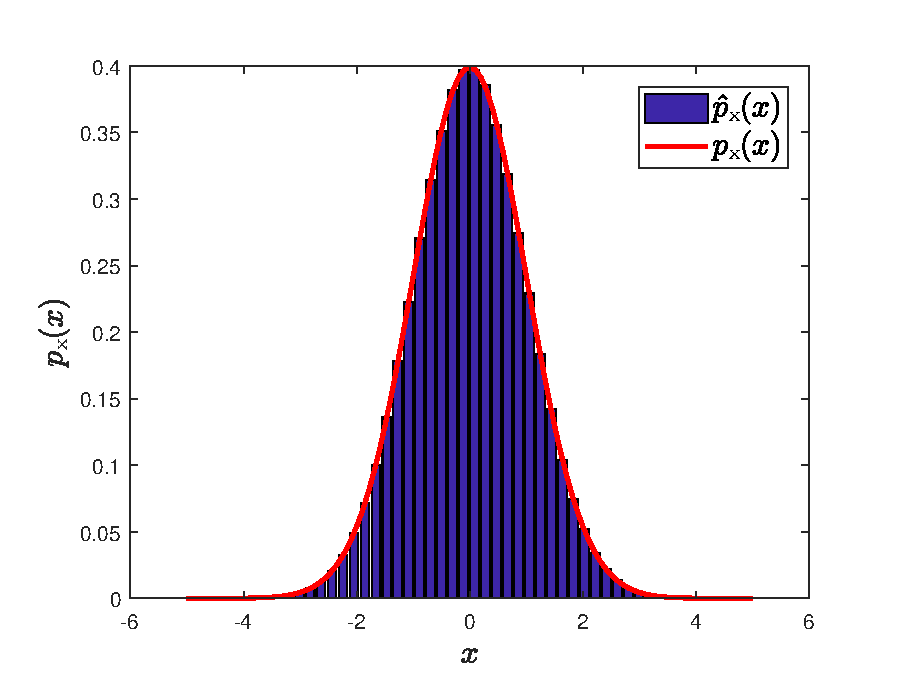
\includegraphics[width = 0.8\textwidth]{pdf_normal.eps}
      \caption{Gaussian PDF and histogram of samples}
      \label{fig:1}
    \end{figure}

  The source code to plot Figure \ref{fig:1} could be found in Appendix \ref{sec:a:code}. Here are the core codes:
  \lstinputlisting[firstline=4,lastline=4, firstnumber=4]{matlabscript.m}
  \lstinputlisting[firstline=6,lastline=7, firstnumber=6]{matlabscript.m}
  To understand line 6, note that if we have $n$ samples of $\rvx$ denoted by $x^{(i)}, i = 1, 2, \cdots, n$, then the probability density function $p_{\rvx}$ could be estimated as
  \begin{equation*}
    \begin{aligned}
      p_{\rvx}(x_0) &= \left.\frac{\mathrm{d}}{\mathrm{d}x} \Prob(\rvx \leq x) \right|_{x = x_0} \\
      &\approx \frac{\Prob(x_0 - \Delta x < \rvx \leq x_0)}{\Delta x}\\
      &\approx \frac{1}{n\Delta x} \sum_{i = 1}^n \1_{x^{(i)} \in (x_0 - \Delta x, x_0]}.
    \end{aligned}    
  \end{equation*}
    
\end{enumerate}
  
  % \newpage
  
  % \appendix
  % \section{Source code}
  % \label{sec:a:code}
  % % \lstlistoflistings
  % Source code for plotting Figure \ref{fig:1} is shown as follows.
  % \lstinputlisting{matlabscript.m}
  
\end{document}
%%% Local Variables:
%%% mode: latex
%%% TeX-master: t
%%% End:
